\documentclass[fleqn,xcolor=table,10pt,final]{beamer}

\setbeamertemplate{footline}[text line]{%
    \parbox{\linewidth}{\vspace*{-8pt}
    \tt{https://github.com/AlbertDeFusco/goldRush}
  \hfill}}
\setbeamertemplate{navigation symbols}{}
\usepackage{amsmath,amsfonts,amssymb,pxfonts,xspace}
\usepackage{textpos}
\usepackage{colortbl}
\usepackage{verbatim}
\usepackage{graphicx}
\usepackage{color}
\usepackage{listings}
\usepackage{tikz}

\definecolor{green}{rgb}{0.1,0.8,0.1}
\definecolor{gold}{rgb}{0.85,.66,0}

\lstset{
    basicstyle=\footnotesize,
    keywordstyle=\color[rgb]{0.1,0.8,0.1}\bfseries,
    commentstyle=\color{blue},
    numbers=left,
    stringstyle=\ttfamily\color{red!50!brown},
    showstringspaces=false}
\lstset{literate=%
   *{0}{{{\color{red!20!violet}0}}}1
    {1}{{{\color{red!20!violet}1}}}1
    {2}{{{\color{red!20!violet}2}}}1
    {3}{{{\color{red!20!violet}3}}}1
    {4}{{{\color{red!20!violet}4}}}1
    {5}{{{\color{red!20!violet}5}}}1
    {6}{{{\color{red!20!violet}6}}}1
    {7}{{{\color{red!20!violet}7}}}1
    {8}{{{\color{red!20!violet}8}}}1
    {9}{{{\color{red!20!violet}9}}}1
}



\begin{document}

\title{Cilk Plus Reducers}
\author{Albert DeFusco}
\date{\today}
\frame{\titlepage}


\begin{frame}
  \frametitle{Parallel Gold Sifting}
  \begin{itemize}
    \item each pan can sift a constant amount of dirt/day
    \item more pans means more dirt sifted
  \end{itemize}
  \vskip 0.2cm
  \begin{itemize}
    \item each pan sifts independently
    \item each pan has a definite amount of dirt to sift
  \end{itemize}
  \vskip 0.2cm
  \begin{itemize}
    \item sifting is parallelizable
  \end{itemize}
\end{frame}

\begin{frame}[fragile]
  \frametitle{Serial Gold Sifting}
  \begin{lstlisting}[language=C++,basicstyle=\scriptsize]
#include <list>
class pan
{
  public:
    pan();          //create array of random integers
    bool hasGold(); //calls sift; true if sift returns >0
    int sift();     //returns frequency of 79 (gold)
}

int main()
{
  std::list<int> withGold;
  pan* myPans = new pan[nPans];

  for(int i=0; i<nPans; ++i)
  {
    bool gold = myPans[i].hasGold();
    if(gold) {
      withGold.push_back(i);
    }
  }
  list<int>::const_iterator iterator;
  for (iterator = withGold.begin(); iterator != withGold.end(); ++iterator)
    cout << *iterator << "  ";
  cout << endl;

  return 0;
}
  \end{lstlisting}
\end{frame}

\begin{frame}[fragile]
  \frametitle{Parallel Gold Sifting}
  \begin{lstlisting}[language=C++,basicstyle=\scriptsize]
#include <list>
class pan
{
  public:
    pan();          //create array of random integers
    bool hasGold(); //calls sift; true if sift returns >0
    int sift();     //returns frequency of 79 (gold)
}

int main()
{
  std::list<int> withGold;
  pan* myPans = new pan[nPans];

  cilk_for(int i=0; i<nPans; ++i)
  {
    bool gold = myPans[i].hasGold();
    if(gold) {
      withGold.push_back(i);
    }
  }
  list<int>::const_iterator iterator;
  for (iterator = withGold.begin(); iterator != withGold.end(); ++iterator)
    cout << *iterator << "  ";
  cout << endl;

  return 0;
}
  \end{lstlisting}
  \begin{tikzpicture}[overlay]
    \draw[color=red] (5.5,2.5) rectangle (0.0,4.5);
  \end{tikzpicture}
\end{frame}
\begin{frame}[fragile]
  \frametitle{Parallel Gold Sifting}
  \begin{lstlisting}[language=C++,basicstyle=\scriptsize]
#include <list>
class pan
{
  public:
    pan();          //create array of random integers
    bool hasGold(); //calls sift; true if sift returns >0
    int sift();     //returns frequency of 79 (gold)
}

int main()
{
  std::list<int> withGold;
  pan* myPans = new pan[nPans];

  cilk_for(int i=0; i<nPans; ++i)
  {
    bool gold = myPans[i].hasGold();
    if(gold) {
      withGold.push_back(i);
    }
  }
  list<int>::const_iterator iterator;
  for (iterator = withGold.begin(); iterator != withGold.end(); ++iterator)
    cout << *iterator << "  ";
  cout << endl;

  return 0;
}
  \end{lstlisting}
  \begin{tikzpicture}[overlay]
    \draw[color=red] (5.5,2.5) rectangle (0.0,4.5);
    \draw[color=blue] (6,2.5) rectangle (10,4.5);
  \end{tikzpicture}
\end{frame}

\begin{frame}
  \frametitle{Thread Safety}
  \begin{itemize}
    \item Unsafe operations
      \begin{itemize}
        \item Multiple threads accessing the same address
          \begin{itemize}
            \item Basic types are not thread safe
            \item STL types are not thread safe
          \end{itemize}
        \item Threads read and write memory at undetermined times
        \item Leads to a race condition
      \end{itemize}
  \end{itemize}
\end{frame}

\begin{frame}
  \frametitle{Race Condition}
  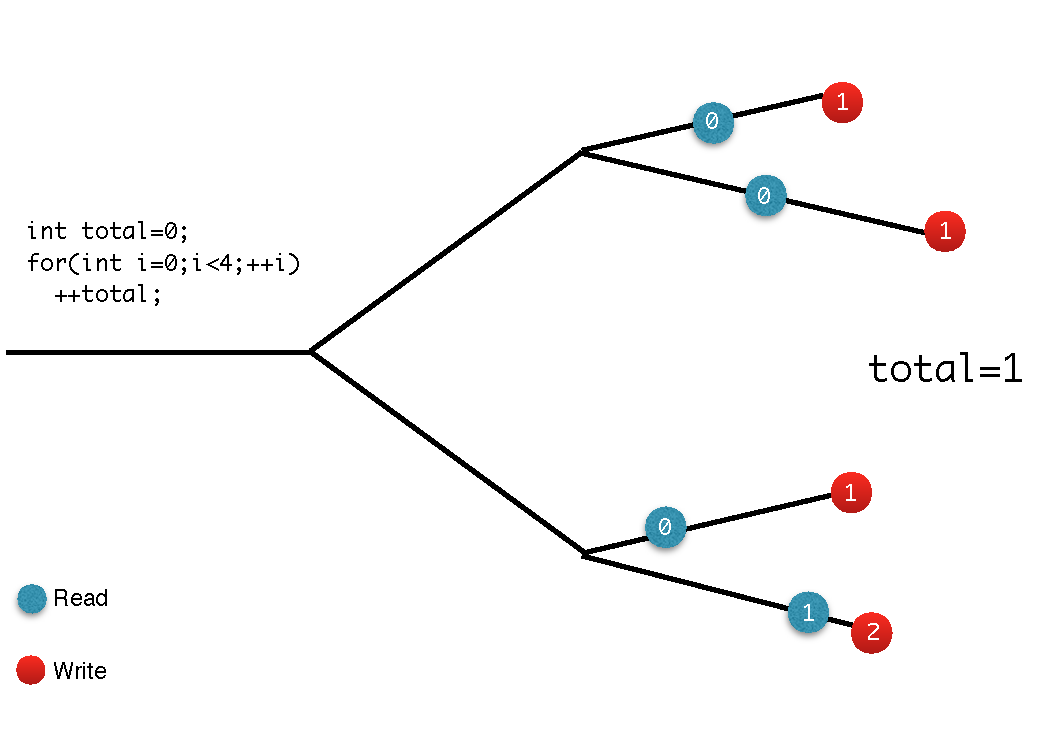
\includegraphics[width=\textwidth]{figures/race}
\end{frame}

\begin{frame}[fragile]
  \frametitle{Inefficient solutions}
  \begin{itemize}
    \item lock
    \item mutex
  \end{itemize}
  \begin{itemize}
    \item cannot use {\tt cilk\_sync} in the loop
      \begin{itemize}
        \item will only sync child threads, not all threads
      \end{itemize}
  \end{itemize}
  \begin{itemize}
    \item break the loop; requiring more storage
  \end{itemize}
  \begin{lstlisting}[language=C++,basicstyle=\scriptsize]
double *sum = new double[N];
cilk_for(int i=0;i<N;++i)
  sum[N] = f(N)
double total=0.0;
for(int i=0;i<N;++i)
  total+=sum[N];
  \end{lstlisting}
\end{frame}

\begin{frame}
  \frametitle{Cilk Reducers}
  \begin{itemize}
    \item Any associative operation is a valid reducer
      \begin{equation*}
        x\ OP\ y = y\ OP\ x
      \end{equation*}
    \item Provide thread safe access to a ``smart pointer''
    \item Small parallel overhead for usage
    \item Very extensible
    \item Operations are guaranteed to execute in the same order as in serial
  \end{itemize}
\end{frame}

\begin{frame}
  \frametitle{Cilk Reducers: views}
  \begin{itemize}
    \item At spawn each strand gets a private ``view'' of the reducer
    \item When strands merge
      \begin{itemize}
        \item ``views'' are combined by $OP$
        \item The combined ``view'' is given to the exit thread
      \end{itemize}
  \end{itemize}
\end{frame}

\begin{frame}
  \frametitle{Cilk Reducers: views}
  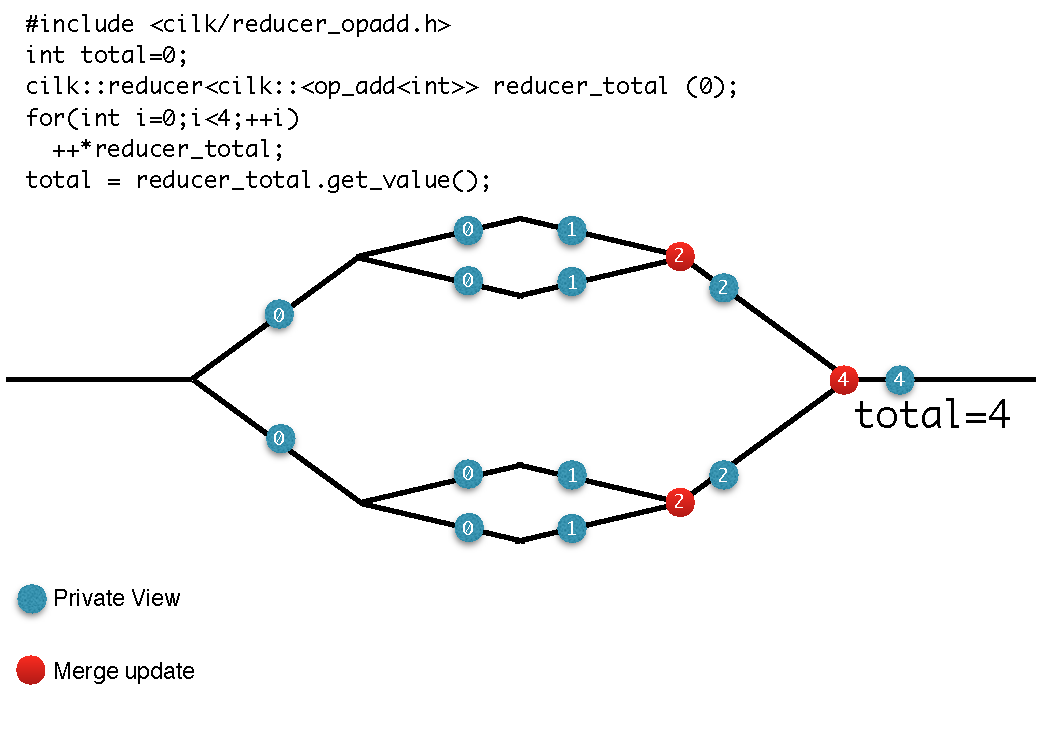
\includegraphics[width=\textwidth]{figures/reduce}
\end{frame}

%\begin{frame}[fragile]
  %\frametitle{Sum reduction}
  %\begin{lstlisting}[language=C++,basicstyle=\scriptsize]
%#include <cilk/cilk.h>
%#include <cilk/reducer_add.h>
%int total;
%cilk::reducer<cilk::op_add> red_total (0);
%cilk_for(int i=0;i<N;++i)
  %*total += f(N);
%total = red_total.get_value();
  %\end{lstlisting}
  %\begin{itemize}
    %\item Direct assignment of a reducer is not allowed
  %\end{itemize}
%\end{frame}

\begin{frame}[fragile]
  \frametitle{Find pans with gold}
  \begin{lstlisting}[language=C++,basicstyle=\scriptsize]
#include <cilk/cilk.h>
#include <cilk/reducer_list.h>

  std::list<int> withGold;
  cilk::reducer< cilk::op_list_append<int> > reducer_withGold;
  pan* myPans = new pan[nPans];

  cilk_for(int i=0; i<nPans; ++i)
  {
    bool gold = myPans[i].hasGold();
    if(gold) {
      reducer_withGold->push_back(i);
    }
  }
  withGold = reducer_withGold.get_value();

  list<int>::const_iterator iterator;
  for (iterator = withGold.begin(); iterator != withGold.end(); ++iterator)
    cout << *iterator << "  ";
  cout << endl;
  \end{lstlisting}
  \begin{tikzpicture}[overlay]
    \draw[color=blue] (0.2,4.8) rectangle (9.3,5.1);
    \draw[color=blue] (0.8,2.8) rectangle (5.5,3.1);
    \draw[color=blue] (0.3,2) rectangle (6.2,2.3);
  \end{tikzpicture}
\end{frame}

\begin{frame}[fragile]
  \frametitle{Gold Rush}
  {\scriptsize
  \begin{verbatim}
Gold Rush!

  12 total kB of dirt
  1000 pans

  Found gold in 15 pans
  Pan IDs: 94  142  265  268  289  440  442  443  569  600  721  781  783  806  818
  \end{verbatim}
}
\end{frame}

\end{document}
